%Car I
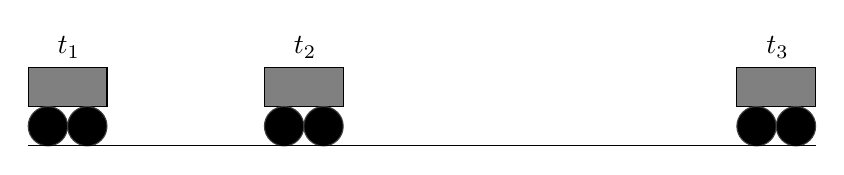
\begin{tikzpicture}
\filldraw[draw = black, fill = gray] (0,0) rectangle (1,0.5);
\filldraw[fill = black, draw = darkgray] (0.25,-0.25) circle (0.25cm);
\filldraw[fill = black, draw = darkgray] (0.75,-0.25) circle (0.25cm);
%Car II
\filldraw[draw = black, fill = gray] (3,0) rectangle (4,0.5);
\filldraw[fill = black, draw = darkgray] (3.25,-0.25) circle (0.25cm);
\filldraw[fill = black, draw = darkgray] (3.75,-0.25) circle (0.25cm);
%Car III
\filldraw[draw = black, fill = gray] (9,0) rectangle (10,0.5);
\filldraw[fill = black, draw = darkgray] (9.25,-0.25) circle (0.25cm);
\filldraw[fill = black, draw = darkgray] (9.75,-0.25) circle (0.25cm);
\draw[black] (0,-0.5) -- (10,-0.5);
\draw[black] (0.25,0.75) node[anchor=west] {$t_1$};
\draw[black] (3.25,0.75) node[anchor=west] {$t_2$};
\draw[black] (9.25,0.75) node[anchor=west] {$t_3$};
\end{tikzpicture}

Acceleration is significant in kinematics and dynamics, particularly 
because of Newton's Laws. From a strictly kinematic perspective, we can interpret Newton’s Laws as saying that a force(which we will not define for now) causes a body to have an acceleration that is a function of time. This is often presented as nothing more than a truth of nature, but it is important to understand that forces do not cause a body to have constant velocity but rather constant acceleration. While this might seem trivial, problems involving this idea are rife in elementary physics. For now, let us define linear acceleration(as opposed to angular or centripetal acceleration; which we will define later). Acceleration is defined as the rate of change of the velocity of an object with respect to time. Before introducing instantaneous acceleration, first, we have to introduce average velocity. Average acceleration is simply the change in velocity for a given time period divided by the length of the small time period. \begin{equation} = \frac{1}{t_2-t_1} \int_{v_1}^{v_2} dv\end{equation} From this definition of average acceleration it is natural to see why we would want to define an instantaneous acceleration just like we wanted to define an instantaneous velocity. This definition begs the question, "What happens as $t_2-t_1$ goes to 0. When we take the limit, we find that instantaneous acceleration can be defined as $$\frac{d\vec{v}}{dt}$$ or as $$\frac{d^2\vec{x}}{dt^2}$$ These two expressions; however, are exactly the same because $$\vec{v}= \frac{d\vec{x}}{dt}$$ so $$\frac{d\vec{v}}{dt} = \frac{d}{dt}\left(\frac{d\vec{x}}{dt}\right) = \frac{d^2\vec{x}}{dt^2}$$ Integrating our definition of velocity over time we find that $\vec{v} = \int \vec{a} \ dt$. While of course in the general case of acceleration, acceleration is changing as a function of time, for most of the problems we will see, acceleration is assumed to be constant. Frankly, we often assume this because if we have a changing acceleration, then the math can get much hairier when dealing with dynamics problems. To give a preview of the future, trying to solve dynamics problems using Newton's first law $\vec{F}=m\vec{a}$ can get quite odd when assuming acceleration to be changing because both the force and acceleration vectors are changing as functions of time. This forces us to use methods of differential equations which is beyond the scope of this book. Now, we can start thinking about motion with constant acceleration. When discussing this topic, there are often a few great formulas that are introduced to solve these types of problems. They are important, but please do not memorize them. They can all be learned and derived from first principles. The first introduction equation is pretty simple \begin{equation} v=v_o+at\end{equation} This equation is saying that the velocity of the object at hand started at a certain fixed velocity and is increasing by a factor of $a$ with time, where $a$ is the velocity of the object. It is important to recognize that often the initial velocity will not be given directly. Instead, the problem will state that a change in velocity has occured over a certain time period. The question may ask for the time period of the velocity change? Here we can write $\Delta v= at$. The second equation is perhaps more hairy, \begin{equation}x = x_0 + v_0 t+\frac{1}{2}at^2\end{equation} If you have already seen Taylor series you can probably guess what the next term would be if the acceleration were changing at a constant rate. The Taylor series is ultimately where this comes from, but we do not need to worry about this here. This equation can be simply derived from the following fact $\vec{x}= \vec{x_0} + \int \vec{v} dt$.  If we have from equation 1 that $v = v_o+at$ we can integrate this with respect to time to find \begin{equation}\Delta x = v_ot+\frac{1}{2}at^2\end{equation} But $\Delta x = x-x_0$, so with rearrangement we arrive at our original equation. The final and perhaps most useful equation for the AP Exam is \begin{equation} v^2=v_0^2+2a \Delta x\end{equation} This comes in very handy when we are not given any information about the time period over which velocity has changed, and we want to find the distance traveled by the object. The derivation is straightforward and can be derived using the first and second equations and nothing else. This will be left as an exercise to the reader because it is important to understand this formula fully. Having formulas to solve constant acceleration problems will prove very useful when we begin problems in which the only force acting on a body is gravity. 
\newline
\newline
\begin{tikzpicture}
\draw (0,0) circle (0.0001cm);
\draw[black] (0,6.5) node[anchor = west] {Position vs Time Graph for Constant Acceleration Motion};
\draw[black] (-1,0) -- (-1,6);
\draw[black] (-1,0) -- (9,0);
\draw (-1,0) parabola (9,6);
\draw[black] (4,-0.5) node[anchor = west] {Time};
\draw[black] (-1.75,3) node[anchor = west] {\begin{turn}{90} Position \end{turn}};
\end{tikzpicture}
\newline